
\chapter{Podstawy teoretyczne}

%\newline\textcolor{orange}{
%Można coś dopisać/ poprawić to powyżej. Chciałem tutaj przedstawić zarys jak wygląda proces.
%myśle żeby poniżej w każdym akapicie opisać krok po kroku jak to wyglądało z użyciem exceli.
%Tylko trzeba to napisać sensownie i łądnie żeby nikt się nie zajebał w akcji i żeby uwzględnić
%wszystkie rzeczy. Tutaj chyba nie będziemy się rozwodzili na temat minusów tego rozwiązania.
%no i potem bym dał informacje na temat użytych technologii: typescript, sharepoint, power au-
%tomate i power apps. imo taka kolejność żeby odzwierciedlała trochę jaki jest proces w apce bo
%bedziesz mógł się odwołąć do poprzednich. np że automate zaciaga dane z SP i każdy wie czym
%jest już sharepoint i essa.}
\section{Struktura procesu}
% Przedmiotem omawianego procesu jest podjęcie decyzji na tematu zakupu usług IT w zakładzie
% Volkswagen Poznań. Polega on na wymianie uwag, dotyczących wcześniej używanego bądź nowego
% oprogramowania, między oddziałem Volkswagen w Poznaniu a zakładem z siedzibą w Wolfsburgu.
Przedmiotem omawianego procesu jest podjęcie decyzji dotyczących zakupu usług IT w zakładzie Volkswagen Poznań. Proces ten polega na wielokrotnej wymianie uwag dotyczących wcześniej używanego lub nowego oprogramowania między oddziałem Volkswagena w Poznaniu a zakładem z siedzibą w Wolfsburgu.

W wyniku wymiany zdań zapada decyzja o zakupie lub rezygnacji z wybranego produktu. Procedura, zazwyczaj podzielona na cztery {indykacje}\footnote{\emph{indykacja}  - wstępne głosowanie}, rozpoczyna się wraz z początkiem czerwca i trwa do końca roku.

Efektem podejmowanych działań jest nabycie odpowiedniej ilości potrzebnych uprawnień licencyjnych. Przy
podejmowaniu decyzji kluczowymi aspektami są:
\begin{itemize}
    \item liczba użytkowników danego oprogramowania,
    \item cena zakupu w porównaniu z rokiem poprzednim,
    \item określenie, czy dana usługa zostanie w pełni wykorzystana biorąc pod uwagę poprzednie kryteria.
\end{itemize}
Dotychczas analiza i przetwarzanie danych odbywały się przy użyciu arkuszy kalkulacyjnych programu Excel, a wymiana informacji między jednostkami była realizowana za pomocą wiadomości e-mail.
\subsection{Gromadzenie danych dotyczących ofert usługodawców}
Informacje na temat serwisów są zbierane na początku roku, przed rozpoczęciem cyklu procesu. W tym czasie, prowadzone są rozmowy między menadżerami odpowiedzialnymi za dane rozwiązanie (\akronim{BSM}, \english{Business Service Manager}) a firmami świadczącymi usługi, w celu otrzymania zaaktualizowanych wiadomości związanych z ich produktami. Na podstawie danych od usługodawców oraz menadżerów, powstaje arkusz, który jest przekazywany do zakładu w Poznaniu.
\subsection{Przygotowanie danych}
Otrzymany arkusz kalkulacyjny, zawiera tabelę o strzukturze kolumn podobnej do tabeli \ref{Headers2022}. Brakuje w nim jednak informacji kluczowych do rozpoczęcia cyklu.
Dlatego pierwszym krokiem jest przygotowanie danych przez osobę nadzorującą proces ze strony odziału w Poznaniu.
Jej zadaniem jest manualne przypisanie numeru określającego miejsce powstawania kosztów, wewnętrznie nazywanego \definicja{MPK}. Numer ten definiuje konkretną jednostkę należącą do obszaru IT, która decyduje o zakupie danego produktu. Ponadto, dodawana jest kolumna, w której znajduje się wyliczona różnica cen między rokiem obecnym a poprzednim, w celu określenia czy koszt wzrósł lub zmalał. Tak przetworzony plik zostaje umieszczony we wspólnej przestrzeni dyskowej, co umożliwia pozostałym uczestnikom procesu przystąpienie do analizy oraz dalszego przetwarzania zawartych w nim informacji.

\renewcommand{\arraystretch}{1.1} % Zwiększenie wysokości komórek
\begin{table}[H] % [H] - tabela dokładnie w tym miejscu
    \begin{adjustwidth}{-50pt}{-20pt}
        \centering
        \caption{Nagłówki kolumn z arkusza kalkulacyjnego z roku 2022}
        \label{Headers2022}
        \makebox[\textwidth][c]{%
            \begin{tabular}{*{3}{|m{1.1cm}}|w|m{0.4cm}|m{1.5cm}|m{1.75cm}|w|m{0.7cm}|w|m{0.7cm}|}
                \hline
                Service group & Service main group & Service sub group & Business Service & ID & Business Service Manager & Unit of Measurement & PL70 2022 PLAN EUR w KVA & QTY & PL71 2023 PLAN EUR w KVA & QTY \\ \hline
            \end{tabular}
        }
    \end{adjustwidth}
\end{table}

\subsection{Przebieg Iteracji}
W trakcie trwania iteracji analizowane są kluczowe informacje, takie jak:
\begin{itemize}
    \item jednostka miary (ang. \emph{Unit of Measurement}),
    \item decyzja podjęta w roku poprzednim,
    \item cena oraz liczba użytkowników w roku obecnym,
    \item cena oraz liczba użytkowników w roku przyszłym.
\end{itemize}
Po analizie i porównaniu danych z wcześniejszych lat, w arkuszu powstają kolejne kolumny. Ich struktura nie jest określona przez żaden standard, ale zazwyczaj zawierają one:
\begin{itemize}
    \item Komentarz wewnętrzny,
    \item Status,
    \item Komentarz klienta.
\end{itemize}

\noindent\emph{Komentarz wewnętrzny} nie jest wymagany dla każdego serwisu. Jest on zapisywany w celu skonsultowania decyzji ze współpracownikami.\\ \emph{Status} określa wstępną, wymaganą decyzję (Zaakceptowany/Niezaakceptowany).\\ \emph{Komentarz klienta} zawiera uzasadnienie podjętej decyzji ze strony Volkswagen Poznań.\\Tak uzupełniony arkusz zostaje przekazany pośrednio przez zakład w Wolfsburgu do zarządu firmy. \par
Kolejnym etapem jest analiza tych informacji przez wcześniej wymienione podmioty. Ich zadaniem jest konfrontacja podjętej decyzji. Dodawane są kolejne kolumny:
\begin{itemize}
    \item Komentarz BSM,
    \item Komentarz K-DES.
\end{itemize}

\noindent\emph{Komentarz BSM} to opinia wyrażona przez menedżera usługi, natomiast \emph{Komentarz K-DES} stanowi odpowiedź międzynarodowego zarządu firmy, który odpowiada za kształtowanie strategii IT.\par
Zaaktualizowany plik powraca do Volkswagen Poznań, rozpoczynając tym samym kolejną iterację procesu.







% Podsumowanie przebiegu proceso - nie tworzyłem nowego pliku na dwa zdania.
\vspace{1cm}
Jak wcześniej wspomniano, proces składa się zazwyczaj z czterech iteracji. Etapem kończącym cykl jest sporządzenie wymaganych dokumentów oraz faktur.

\section{Wykorzystane technologie}
Aby usprawnić przebieg procesu, zabiezpieczyć go przed błędami i usystematyzować, stworzona została aplikacja do jego obsługi. Głównym kryterium przy doborze technologii była powszechna dostępność do powstałego systemu wśród pracowników. Dlatego też zdecydowano się na wykorzystanie komponentów pakietu \emph{Office 365}. Pakiet ten jest bardzo rozbudowany i jest powszechnie używany w firmie Volkswagen. Zawiera on programy pozwalające na stworzenie kompletnego systemu bez konieczności dostępu do dodatkowych usług.
\subsection{Skrypty pakietu Office}
Skrypty pakietu Office pozwalają na automatyzacje zadań w arkuszach kalkulacyjnych Excel. Jedną z dostępnych opcji jest  funkcja \emph{Action Recorder}, która daje możliwość "nagrania" sekwencji kroków wykonanych przez użytkownika, a następnie przekształca je na skrypt wielokrotnego użytku.\par
Skrypty pakietu Office dysponują również wbudowanym \emph{edytorem kodu} (\english{Code Editor}), opartym na języku \emph{TypeScript}, będącym odmianą \emph{JavaScript}. Sam edytor, choć stosunkowo ograniczony, umożliwia zastosowanie konstrukcji niedostępnych w Action Recorder, takich jak instrukcje warunkowe czy pętle.\par
Ponadto program Excel pozwala na zapis skryptu w skoroszycie. Oznacza to, że każdy użytkownik dysponujący dostępem do pliku uzyskuje również możliwość uruchomienia kodu powiązanego ze skoroszytem, do którego jest on przypisany.
\subsection{SharePoint}
SharePoint to platforma wchodząca w skład pakietu Microsoft 365, która służy do zarządzania dokumentami oraz umożliwia efektywną współpracę zespołową. Dzięki niej użytkownicy mogą tworzyć i korzystać z własnych przestrzeni roboczych online, takich jak listy czy archiwa plików, co znacząco ułatwia organizację oraz szybki dostęp do danych.

Listy sharepointowe mogą pełnić funkcję prostych baz danych, które można łatwo zintegrować z takimi narzędziami jak PowerApps, PowerAutomate, czy Excel. Takie rozwiązanie umożliwia dynamiczne aktualizowanie i synchronizowanie danych w czasie rzeczywistym.



\subsection{Power Automate }
Power Automate to narzędzie wchodzące w skład pakietu Microsoft 365, które umożliwia automatyzację procesów biznesowych (\akronim{RPA}, \english{Robotic Process Automation}). Pozwala ono na~tworzenie przepływów pracy (\english{flows}), automatyzujących powtarzalne zadania i integrujących różne systemy, zwiększając efektywność procesów biznesowych.

Flow w Power Automate jest odpowiednikiem funkcji w standardowych językach programowania. Na przykład przepływ może automatycznie wysyłać powiadomienia e-mail po aktualizacji rekordu w SharePoint. Różnica polega na tym, że jest on tworzony w wizualnym środowisku Low-Code i~działa na zasadzie logicznego ciągu akcji wyzwalanych kolejno przez określone instrukcje.

Za pomocą flow można tworzyć własne procesy, które przy odpowiedniej implementacji, dorównują tym znanym z pełnych środowisk kodowych pod względem logiki i efektywności. Do dyspozycji są instrukcje warunkowe, pętle, zmienne, operacje na danych czy integracje z API poprzez konektory \texorpdfstring{\cite{v-aangie_official_nodate}}{}.

\subsection{Power Apps}

Power Apps to środowisko Low-Code'owe, wchodzące w skład pakietu Office 365, które jest dedykowanym rozwiązaniem do tworzenia aplikacji biznesowych. Dzięki intuicyjnemu interfejsowi graficznemu daje możliwość prostej implementacji mechanizmu działania nawet przez osoby bez zaawansowanej wiedzy programistycznej. Jest ona zintegrowana z innymi usługami pakietu Office 365, takimi jak SharePoint czy Power Automate, co rozszerza możliwości stworzonych aplikacji.

Power Apps pozwala na stworzenie spersonalizowanej aplikacji, dostosowanej do motywu organizacji, a przy połączeniu z innymi serwisami daje możliwość tworzenia zaawansowanych rozwiązań, minimalizując przy tym czas potrzebny na ich zaimplementowanie.

Ekrany aplikacji, komponowane za pomocą tego rozwiązania, porównywalne są z tymi, które można stworzyć w standardowych środowiskach programistycznych (jak np. JavaScript czy .NET), jednak proces ich tworzenia jest prostszy, ze względu na obecność edytora wizualnego. Umożliwia on korzystanie z gotowych komponentów w aplikacji, takich jak przyciski, pola danych wejściowych, listy, tabele, grafiki etc.

Dodawanie elementów do ekranów aplikacji odbywa się poprzez przeciąganie ich z biblioteki i upuszczanie w wybranym miejscu. Każdy komponent, może zostać skonfigurowany według potrzeb użytkownika poprzez edycje \emph{właściwości}. Możemy określić między innymi wypełnienie czy pozycję \emph{X} i \emph{Y} na ekranie, ale niektóre obiekty mają też unikalne właściwości takie jak \emph{OnSelect} \footnote{OnSelect -- określa akcje, które zostaną wykonane po naciścięciu elementu} dla przycisku.


\newpage

\begin{figure}[h] % h - tu, t - góra, b - dół, p - strona dodatkowa
    \centering
    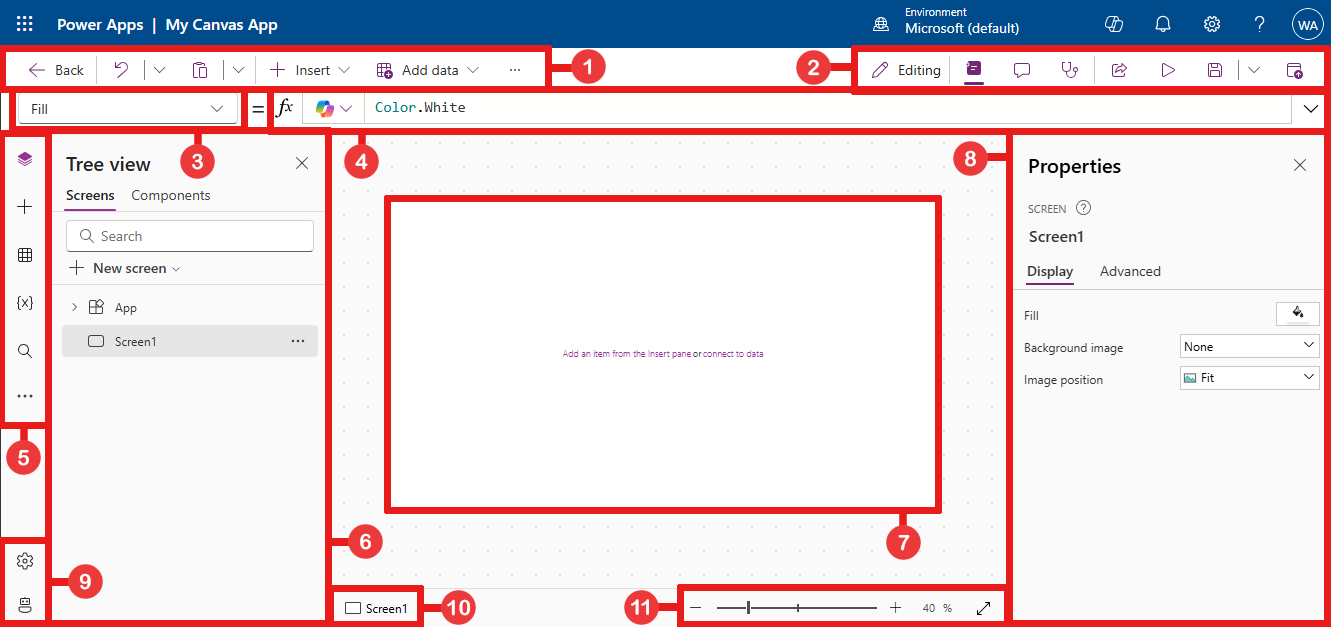
\includegraphics[width=\textwidth]{figures/PowerAppsOverview}
    \caption{Edytor Power Apps}
    \label{fig:PowerAppsEditorOverview}
\end{figure}
\textcolor{red}{LINK DO OBRAZKA I OPISU ELEMENTÓW: https://learn.microsoft.com/en-us/power-apps/maker/canvas-apps/power-apps-studio}

Rysunek \ref{fig:PowerAppsEditorOverview} przedstawia edytor programu. Zawiera on następujące elementy:
\begin{enumerate}
    \item \textbf{Pasek poleceń:} wyświetla inny zestaw poleceń w zależności od wybranego kontrolki.
    \item \textbf{Akcje aplikacji:} Opcje wyświetlania właściwości, dodawania komentarzy, sprawdzania błędów, udostępniania, podglądu, zapisu lub publikowania aplikacji.
    \item \textbf{Lista właściwości:} Lista właściwości wybranego obiektu.
    \item \textbf{Pasek formuł:} Tworzenie lub edycja formuły dla wybranej właściwości z użyciem jednej lub więcej funkcji.
    \item \textbf{Menu tworzenia aplikacji:} Panel wyboru umożliwiający przełączanie się między źródłami danych oraz wstawianie dodatkowych opcji.
    \item \textbf{Lista elementów aplikacji:} Pokazuje lementy obecne na ekranie w postaci drzewa.
    \item \textbf{Płótno/ekran:} Główne płótno do komponowania struktury aplikacji.
    \item \textbf{Panel właściwości:} Lista właściwości wybranego obiektu.
    \item \textbf{Ustawienia i wirtualny agent:} Ustawienia aplikacji lub uzyskanie pomocy od wirtualnego agenta.
    \item \textbf{Selektor ekranu:} Przełączanie się między różnymi ekranami w aplikacji.
    \item \textbf{Zmiana rozmiaru płótna:} Zmienianie rozmiaru wyświetlanego płótna podczas tworzenia aplikacji.
\end{enumerate}











\renewcommand{\arraystretch}{1.5} % Zwiększenie wysokości komórek
\begin{table}[H] % [t] - tabela bliżej górnej krawędzi strony
   \centering
   \caption{}
   \label{HeaderComparison}
   \makebox[\textwidth][c]{%
      \begin{tabular}{|c|W|W|W|}
         \hline
          & \textbf{2022}            & \textbf{2023}            & \textbf{2024}            \\ \hline
         \multirow{12}{*}{\rotatebox{90}{\parbox{4cm}{\centering \textbf{Nazwy kolumn na   \\przestrzeni lat}}}}
          & Service group            & Service group            & Service group            \\ \cline{2-4}
          & Service main group       & Service main group       & Service main group       \\ \cline{2-4}
          & Service sub group        & Service sub group        & Service sub group        \\ \cline{2-4}
          & Business Service         & Business Service         & Business Service         \\ \cline{2-4}
          & ID                       & ID                       & ID                       \\ \cline{2-4}
          & Business Service Manager & Business Service Manager & Business Service Manager \\ \cline{2-4}
          & Unit of Measurement      & Unit of Measurement      & Resource Unit            \\ \cline{2-4}
          &                          & Settlementtype           & Settlementtype           \\ \cline{2-4}
          & PL71 2023 PLAN EUR w KVA & PL71 2023 PLAN EUR w KVA & PL72 2024 PLAN EUR w KVA \\ \cline{2-4}
          & QTY                      & QTY                      & QTY                      \\ \cline{2-4}
          & PL71 2023 PLAN EUR w KVA & PL72 2024 PLAN EUR w KVA & PL73 2025 PLAN EUR w KVA \\ \cline{2-4}
          & QTY                      & QTY                      & QTY                      \\ \hline
      \end{tabular}
   }
\end{table}





